\documentclass[10pt]{article}
%----------Packages----------
\usepackage[utf8]{inputenc}
\usepackage[landscape,left=5mm,right=5mm,top=7mm,bottom=7mm]{geometry}
\usepackage{amsmath,amssymb}
\usepackage{multicol}
\usepackage{multirow}
\usepackage{blindtext}
\usepackage{graphicx}
\usepackage[shortlabels]{enumitem}

%----------Page formatting----------
\pagenumbering{gobble}
\setlength{\parindent}{0pt}
\setlength{\parskip}{2pt}
\renewcommand\labelitemi{$\vcenter{\hbox{\tiny$\bullet$}}$}

%----------Symbols----------
\newcommand{\ep}{\varepsilon}

%----------General----------
\newcommand{\ds}{\displaystyle}
\newcommand{\tab}{\hspace{.02\textwidth}}
\newcommand{\twoEqn}[4]{$\makebox[#3][l]{$#1$} \makebox[#4][l]{$#2$}$}
\newcommand{\threeEqn}[6]{$\makebox[#4][l]{$#1$} \makebox[#5][l]{$#2$} \makebox[#6][l]{$#3$}$}
\newcommand{\splittab}{\hspace{2.58ex}}

%----------Math----------
\renewcommand{\d}{\,\mathrm{d}}
\newcommand{\inv}{^{-1}}

%----------Brackets----------
\newcommand{\lrb}[1]{\left(#1\right)}
\newcommand{\sqb}[1]{\left[#1\right]}
\newcommand{\abs}[1]{\left|#1\right|}
\let\originalleft\left
\let\originalright\right
\renewcommand{\left}{\mathopen{}\mathclose\bgroup\originalleft}
\renewcommand{\right}{\aftergroup\egroup\originalright}

%----------Sections----------
\makeatletter
\renewcommand{\section}{\@startsection{section}{1}{0ex}
                                {-2ex}
                                {0.7ex}
                                {\normalfont\large\bfseries}}
\renewcommand{\subsection}{\@startsection{subsection}{2}{0ex}
                                {-0.4ex}
                                {0.4ex}
                                {\normalfont\normalsize\bfseries}}
\makeatother
\setcounter{secnumdepth}{0}

%----------MECH 260----------
\newcommand{\surf}{\text{surf}}
\newcommand{\upward}{\text{upward}}
\newcommand{\CW}{\text{CW}}
\newcommand{\NA}{\text{NA}}
\renewcommand{\max}{\text{max}}
\renewcommand{\min}{\text{min}}
\newcommand{\nom}{\text{nom}}
\newcommand{\total}{\text{total}}
\newcommand{\Y}{\text{Y}}
\newcommand{\s}{\text{s}}
\newcommand{\UT}{\text{UT}}
\newcommand{\UC}{\text{UC}}
\newcommand{\Tresca}{\text{Tresca}}
\newcommand{\vM}{\text{vM}}
\newcommand{\Mohr}{\text{Mohr}}
\newcommand{\inside}{\text{inside}}
\newcommand{\outside}{\text{outside}}
\newcommand{\ax}{\text{ax}}
\newcommand{\cyl}{\text{cyl}}
\newcommand{\sph}{\text{sph}}

%----------Document Begins Here----------
\begin{document}

\begin{center}
    \LARGE{\textbf{MECH 260 Formula Sheet}}
\end{center}

\begin{multicols*}{3}

\section{General Loading}

Stress and Strain:

\tab\twoEqn{\ds\sigma=\frac{F}{A}}{\ds\ep=\frac{\delta}{L_0}}{10em}{10em}

Young's Modulus:

\tab\twoEqn{\ds E=\frac\sigma\ep}{\ds\delta=\frac{FL_0}{AE}}{10em}{10em}

Poisson's Ratio:

\tab $\ds\ep_{y,z}=\frac{-\nu}{E}\sigma_x$

Hooke's Law:

\tab $\ds\ep=\frac 1E\sqb{\sigma_{\parallel}-\nu\lrb{\sigma_{\perp 1}+\sigma_{\perp 2}}}+\alpha_L\Delta T$

Rearranged Hooke's Law:

\tab $\ds\sigma=\lrb{\frac{E}{(1+\nu)(1-2\nu)}}\sqb{(1-\nu)\ep_{\parallel}-\nu\lrb{\ep_{\perp 1}+\ep_{\perp 2}}}$

\tab $\ds-\lrb{\frac{E}{1-2\nu}}\alpha_L\Delta T$

Volumetric Strain:

\tab $\ep_v\approx\ep_x+\ep_y+\ep_z$

Bulk Modulus:

\tab {\small$\ds\lrb{\frac{\sigma_x+\sigma_y+\sigma_z}{3}}=\underbrace{\frac{E}{3(1-2\nu)}}_K\Big[\lrb{\ep_x+\ep_y+\ep_z}-3\alpha_L\Delta T\Big]$}

Shear Stress and Strain:

\tab\twoEqn{\ds\tau=\frac VA}{\ds\gamma=\frac\delta L}{10em}{10em}

Shear Stress:

\tab $\ds\tau_{xy}$ means stress on $x$ plane in $y$ direction

Shear Strain:

\tab $\gamma_{xy}$ is angle by which $(+x,+y)$ scissors close

Shear Modulus:

\tab $\ds\tau_{xy}=G\gamma_{xy}$

Table of Elastic Constants: \medskip

\begingroup
\renewcommand{\arraystretch}{1.4}
$\begin{array}{ccccc}
    \hline
    & \multicolumn{4}{c}{\text{Find}} \\ \cline{2-5}
    \text{Without} & E & \nu & G & K \\ \hline
    E & & \frac{3K-2G}{6K+2G} & \frac{3K(1-2\nu)}{2(1+\nu)} & \frac{2G(1+\nu)}{3(1-2\nu)} \\
    \nu & \frac{9KG}{G+3K} & & \frac{3EK}{9K-E} & \frac{EG}{9G-3E} \\
    G & 3K(1-2\nu) & \frac 12-\frac{E}{6K} & & \frac{E}{3(1-2\nu)} \\
    K & 2G(1+\nu) & \frac{E}{2G}-1 & \frac{E}{2(1+\nu)} & \\ \hline
\end{array}$
\endgroup

\newcolumn

\section{Stress Concentration}

Nominal Stress:

\tab $\ds\sigma_\nom=\frac{F}{A_\text{min}}$

Stress Concentration:

\tab $\ds K=\frac{\sigma_\max}{\sigma_\nom}$

Factor of Safety (Ductile):

\tab $\ds\abs{\sigma_\nom}=\frac{\sigma_\Y}{f_\s}$

Factor of Safety (Brittle):

\tab $\ds\abs{\sigma_\max}=\begin{cases}
    \frac{\sigma_\UT}{f_\s} & \text{Tension} \\
    \frac{\sigma_\UC}{f_\s} & \text{Compression}
\end{cases}$

Failure:

\tab $\ds f\s\le 1$

\section{Torsion}

Torsion Compatibility:

\tab\twoEqn{\ds\gamma_\surf=\frac{r_\surf}{L}\phi}{\ds\gamma(r)=\frac rL\phi}{10em}{10em}

Torsion Hooke's Law:

\tab\twoEqn{\ds\tau_\surf=\frac{Gr_\surf}{L}\phi}{\ds\tau(r)=\frac{Gr}{L}\phi}{10em}{10em}

Second Polar Moment of Area:

\tab $\ds T=\int_{A_\perp}r\cdot\tau(r)\d A=\frac{G\phi}{L}\underbrace{\int_{A_\perp}r^2\d A}_{J}$

\tab $\ds J=\begin{cases}
    \frac{\pi}{2}r_\surf^4 & \text{Solid Shaft} \\
    \frac{\pi}{2}\lrb{r_\surf^4-r_{\text{in}}^4} & \text{Hollow Shaft} \\
    2\pi tr_\surf^3 & \text{Thin Tube } (t/r_\surf\lesssim 0.01)
\end{cases}$

Torsion Summary:

\tab $\ds\frac{\tau(r)}{r}=\frac TJ=\frac GL\phi$

Horsepower:

\tab $\ds \mathrm{HP}=\frac{\mathrm{RPM}\cdot T}{5252}$

Gears:

\tab\twoEqn{\ds\frac{T_1}{r_1}=\frac{T_2}{r_2}}{r_1\phi_1=-r_2\phi_2}{10em}{10em}

Pulleys:

\tab\twoEqn{T=\lrb{F_1-F_2}r}{\delta_1=\delta_2=r\phi}{10em}{10em}

\newcolumn
\section{Bending}

Shear (downward):

\tab $\ds V(z)=\int_0^z w_\upward(z)\d z+\sum_0^z F_\upward(z)$

Moment (counterclockwise):

\tab $\ds M(z)=\int_0^z V(z)\d z+\sum_0^z T_\CW(z)$

Neutral Axis:

\tab $\ds y_\NA^*=\frac{1}{A_\perp}\int_{A_\perp}y^*\d A$

\tab $\ds y_\NA^*=\frac{1}{A_\total}\sum_{i=1}^n y_{\text{NA},i}^*\cdot A_i$

Second Rectangular Moment of Area:

\tab $\ds M=\int_{A_\perp}\lrb{-y\cdot\sigma_z(y)}\d A=\frac E\rho\underbrace{\int_{A_\perp}y^2\d A}_{I_x}$

\tab $\ds I_x=\int_{y_\min^*}^{y_\max^*}\lrb{y^*-y_\NA^*}^2\cdot w(y^*)\d y^*$

\tab $\ds I_x=\int_{y_\min^*}^{y_\max^*}\lrb{y^*}^2\cdot w(y^*)\d y^*-A_{\perp}\lrb{y_\NA^*}^2$

\tab $\ds I_x=\sum_{i=1}^n I_{B_i,i}+\sum_{i=1}^n A_i\lrb{y_\NA^*-y_{B_i}^*}^2$

\tab $\ds I_x=\begin{cases}
    \frac{bh^3}{12} & \text{Rectangle} \\
    \frac{bh^3}{36} & \text{Triangle} \\
    \frac\pi 4r^4 & \text{Circle} \\
    \lrb{\frac\pi 8-\frac{8}{9\pi}}r^4 & \text{Semi-Circle}
\end{cases}$

Pure Bending Summary:

\tab $\ds\frac{\sigma_z(y)}{-y}=\frac{M}{I_x}=\frac{E}{\rho}$

Composite Bending:

\tab\twoEqn{\ds w_{\text{scaled}}=w\cdot\frac{E}{E_\text{ref}}}{\ds\sigma=\sigma_{\text{scaled}}\cdot\frac{E}{E_\text{ref}}}{10em}{10em}

\section{Stress Transformation and Failure Criteria}

Plane Stress Transformation:

\tab $\ds\sigma_{x'}=\lrb{\frac{\sigma_x+\sigma_y}{2}}+\lrb{\frac{\sigma_x-\sigma_y}{2}}\cos 2\theta+\tau_{xy}\sin 2\theta$

\tab $\ds\sigma_{y'}=\lrb{\frac{\sigma_x+\sigma_y}{2}}-\lrb{\frac{\sigma_x-\sigma_y}{2}}\cos 2\theta-\tau_{xy}\sin 2\theta$

\tab $\ds\tau_{x'y'}=-\lrb{\frac{\sigma_x-\sigma_y}{2}}\sin 2\theta+\tau_{xy}\cos 2\theta$

Mohr's Circle:

\tab\threeEqn{x: (\sigma_x,-\tau_{xy})}{y: (\sigma_y,+\tau_{xy})}{k: (\sigma_k,\tau_k)}{8em}{8em}{5em}

Principal Stresses:

\tab $\ds\tan 2\theta_i=\frac{2\tau_{xy}}{\sigma_x-\sigma_y}$

\tab $\ds\sigma_i=\lrb{\frac{\sigma_x+\sigma_y}{2}}\pm\sqrt{\lrb{\frac{\sigma_x-\sigma_y}{2}}^2+\tau_{xy}^2}$

Tresca Criterion:

\tab $\ds f_\s^\Tresca=\frac{\sigma_\Y/2}{\tau_\max}$

\tab $\ds\max(\sigma_1,\sigma_2,\sigma_3)-\min(\sigma_1,\sigma_2,\sigma_3)=\frac{\sigma_\Y}{f_\s^\Tresca}$

Von Mises Criterion:

\tab $\ds\frac 12\sqb{(\sigma_1-\sigma_2)^2+(\sigma_2-\sigma_3)^2+(\sigma_3-\sigma_1)^2}=\lrb{\frac{\sigma_\Y}{f_\s^\vM}}^2$

Comparison of Tresca and von Mises:

\tab\twoEqn{f_\s^\vM\ge f_\s^\Tresca}{\ds f_\s^\vM\le\frac{2}{\sqrt 3}f_\s^\Tresca}{10em}{10em}

Mohr Criterion:

\tab $\ds\frac{\max(\sigma_1,\sigma_2,\sigma_3)}{\sigma_\UT}-\frac{\min(\sigma_1,\sigma_2,\sigma_3)}{\abs{\sigma_\UC}}=\frac{1}{f_s^\Mohr}$

Gauge Pressure:

\tab\twoEqn{P=P_\inside-P_\outside}{P=\rho gh}{14em}{8em}

Thin-Walled Vessels ($t/r\lesssim 0.1$):

\tab\threeEqn{\ds\sigma_\ax=\frac{Pr}{2t}}{\ds\sigma_\theta^\cyl=\frac{Pr}{t}}{\ds\sigma_\theta^\sph=\frac{Pr}{2t}}{8em}{8em}{6em}

\section{Tips}
\begin{enumerate}[itemsep=0pt, topsep=0pt]
    \item Sign convention for $\sigma$ (compressive is negative)
    \item Gears: $r_1\phi_1=-r_2\phi_2$ (not $\phi_1=-\phi_2$)
    \item Sign convention for $V(z)$ and $M(z)$
    \item $\sigma_{\nom}$ vs. $\sigma_{\max}$
    \item Radius vs. diameter for torsion and bending
    \item Check $t/r\lesssim 0.1$ for thin-walled vessels
\end{enumerate}

\newcolumn
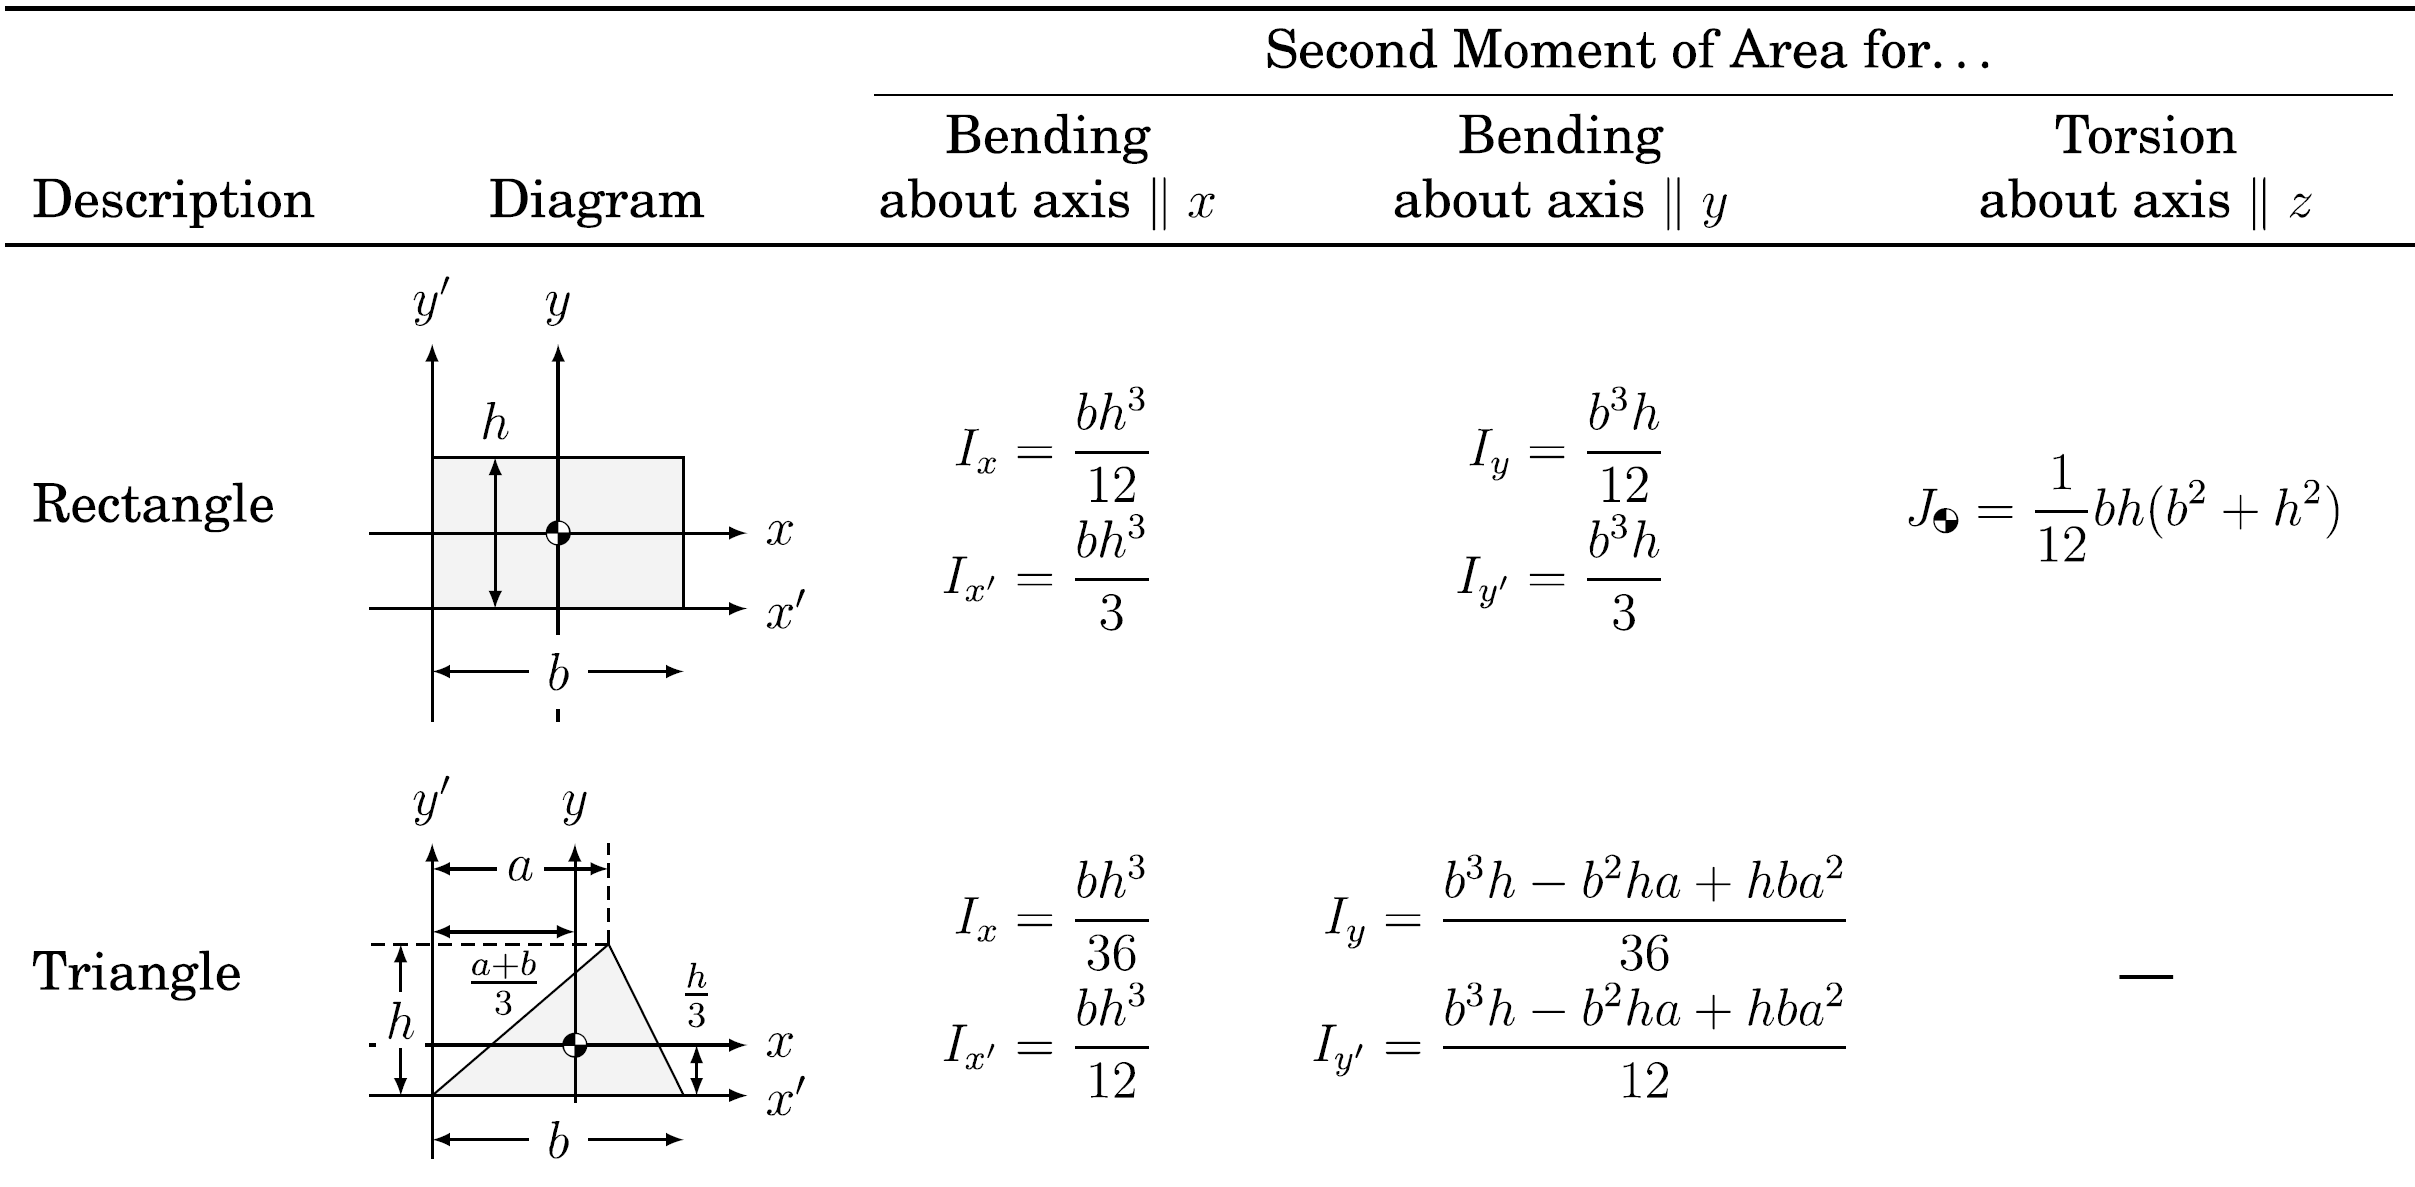
\includegraphics[width=0.61\textwidth]{images/moments_of_area_1.png}
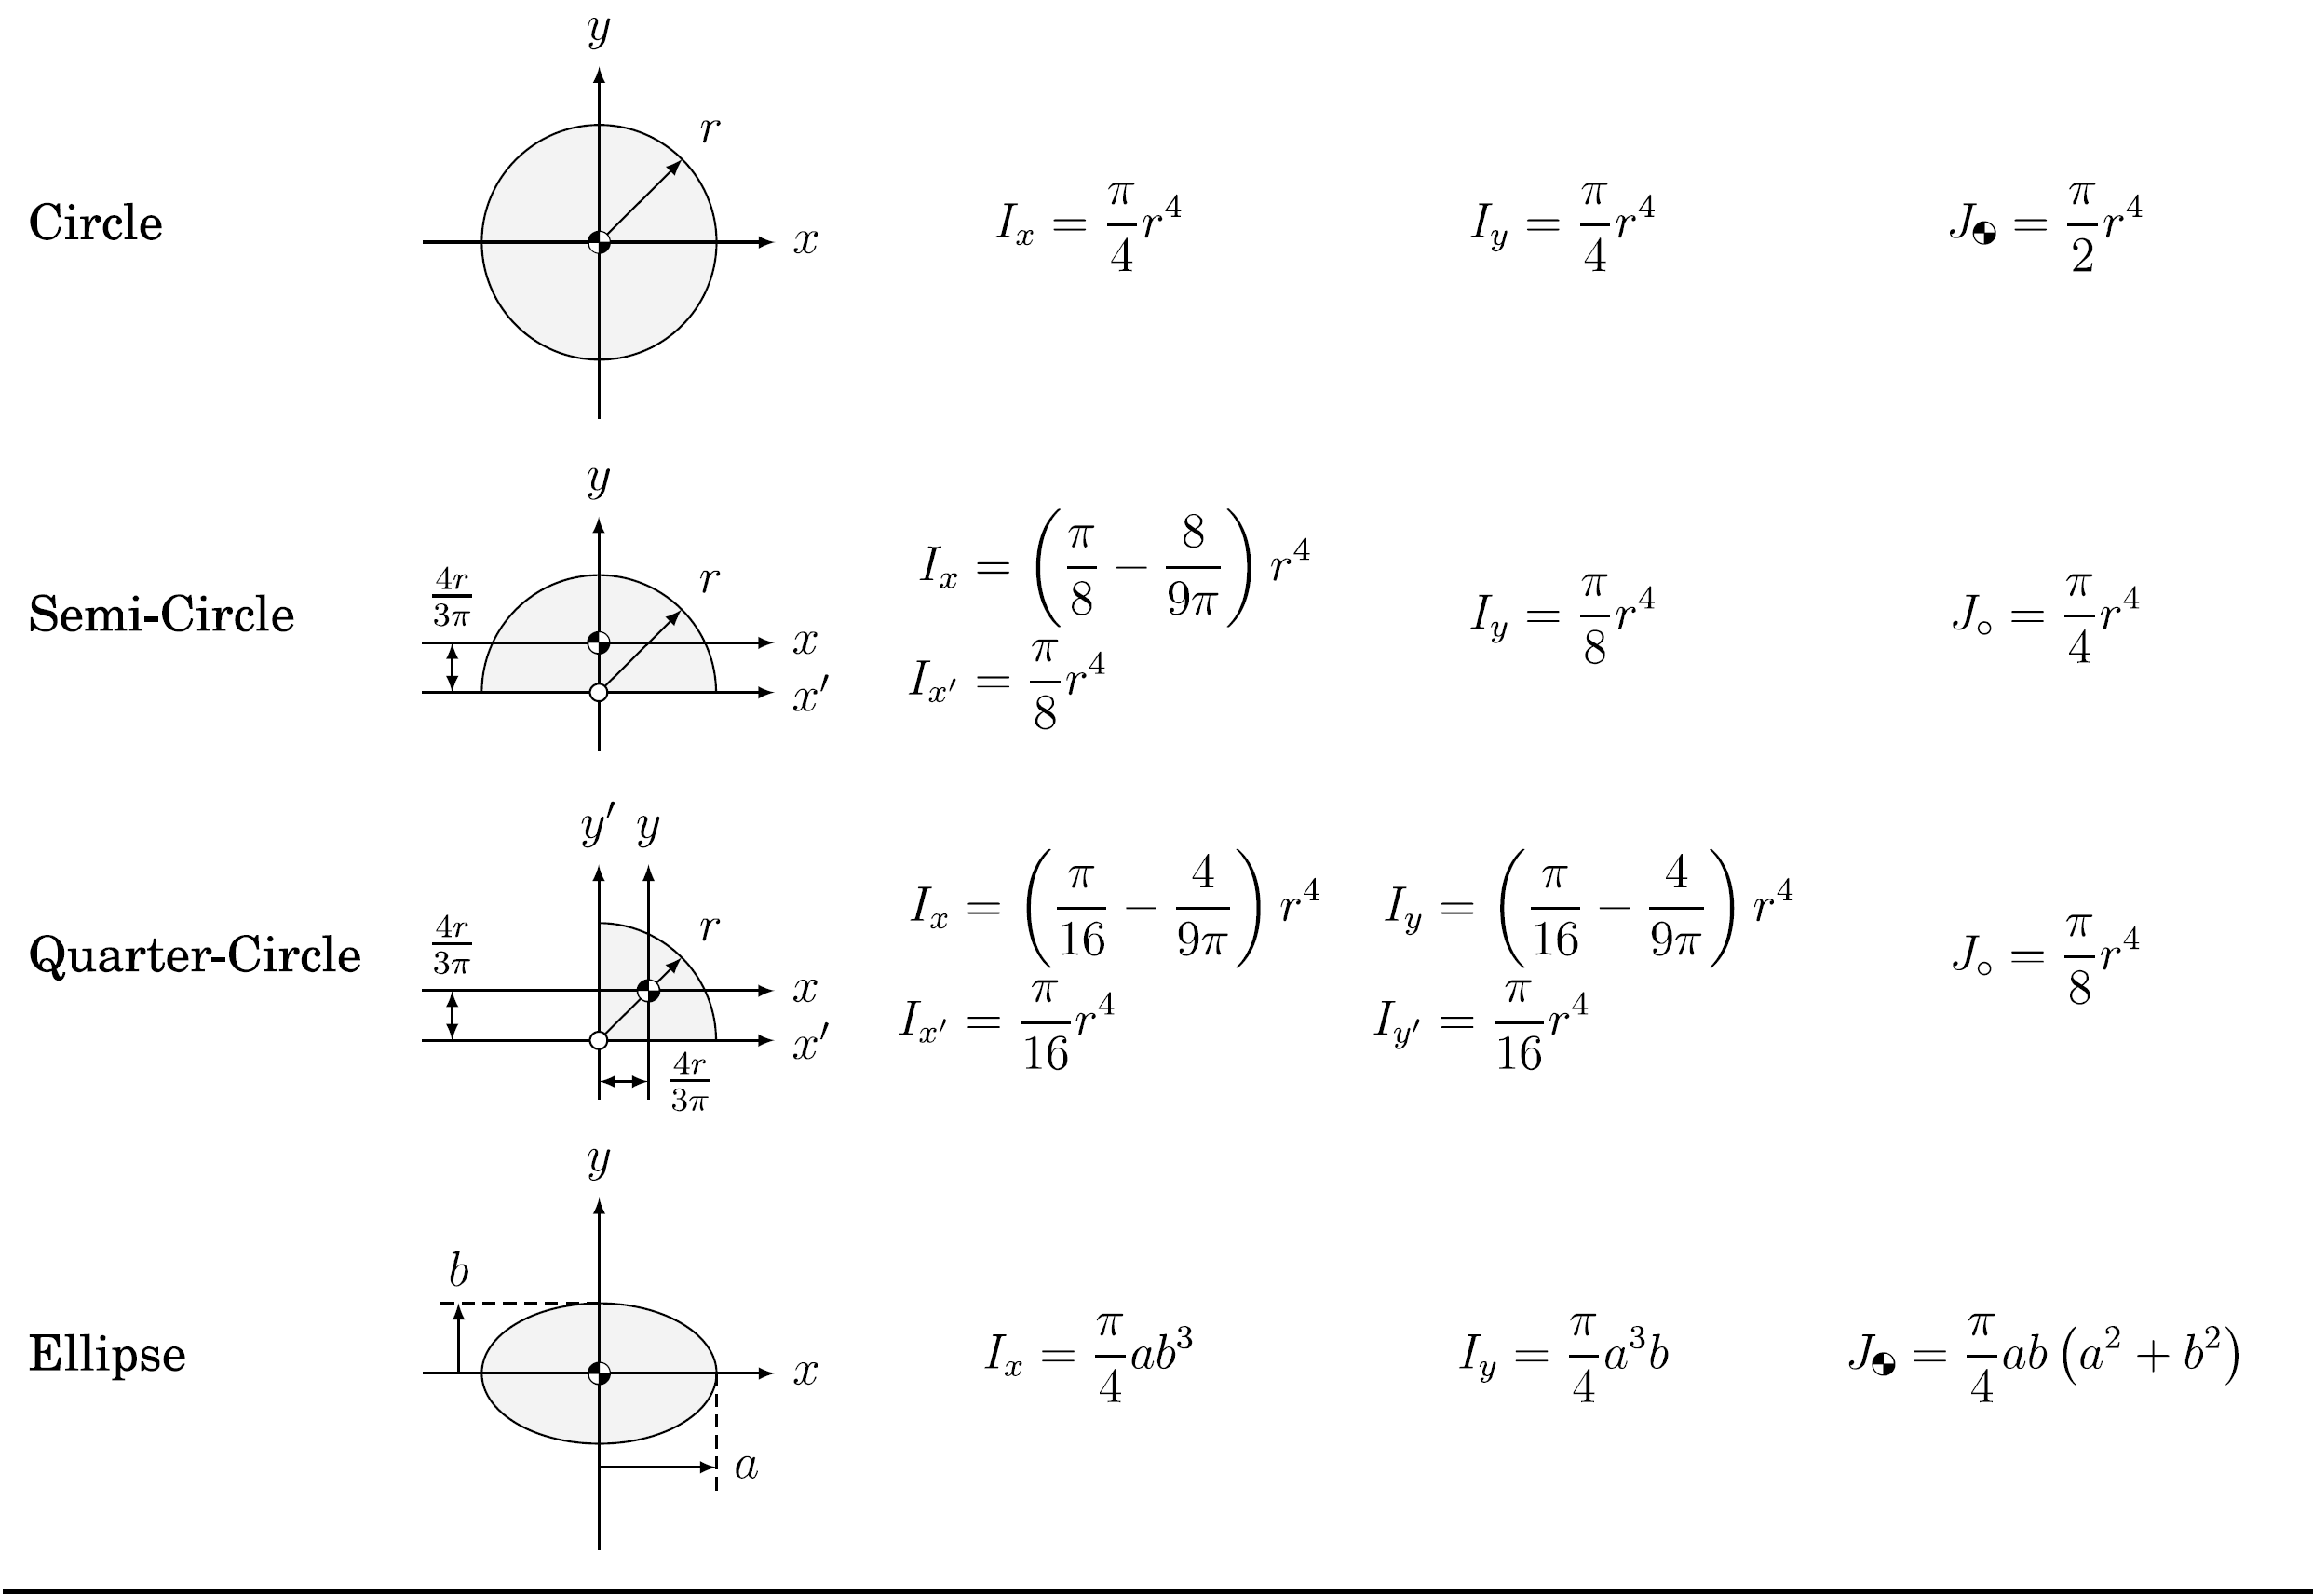
\includegraphics[width=0.61\textwidth]{images/moments_of_area_2.png}

% \rule{\linewidth}{0.1pt}

\scriptsize 
Compiled \today

\end{multicols*}

\end{document}